\documentclass[11pt,a4paper]{article}
\usepackage{color}
\usepackage{enumitem}
\usepackage{fullpage}
\usepackage{graphicx}
\usepackage[colorlinks=true, linkcolor=blue]{hyperref}
\usepackage{setspace}
\usepackage{subfigure}
\usepackage{url}
\setstretch{1.1}

\begin{document}
\title{NNBot: A Robocode Agent of Nothing New}
\author{Libo Yin\\The University of Western Australia}
\maketitle

\section{Background}

The idea of a learning Robocode agent is nothing new. Putting aside counting-based statistical learning techniques such as wave surfing \cite{wave_surfing} and guess factor targeting \cite{guess_factor}, previous studies have demonstrated learning bots using genetic algorithm \cite{ga_robocode}, genetic programming (decision tree) \cite{gp_robocode}, reinforcement learning \cite{reinforcement_robocode}, and neural network. Among all these techniques, neural network is the only one that has been widely accepted by the Robocode community, while the others remain academic. Because neural networks are theoretically able to learn arbitrarily complex unknown functions, they are mostly used for targeting \cite{neural_targeting}, i.e.\ time-series prediction of the future movement of the enemy.

The performance of neural-targeting is a mixture of good and bad. On the good side, these bots have some creative advantages.\ \emph{Gaff}, for example, is one of the best anti-surfers so far. It maintains two neural networks, one trained with short-term history, the other trained with long-term history. The target is chosen as a combination of the output of both neural networks. On the bad side, though, the top of the RoboRumble board is still dominated by hand-coded bots, mostly using different forms of wave surfing and guess factor targeting.

Meanwhile, academic attempts to build Robocode agents concentrate on the application of specific techniques, putting aside domain knowledge. Personally, I'd very much like to know whether or not these bots have demonstrated any creative dynamics that are not available to hand-coded bots. Unfortunately, the authors seem not quite interested in this.

\section{Ideas and Attempts}

The temporal nature of the Robocode game decided that a learning bot must be able to learn the optimal policy as fast as possible during the game without pausing it, and should be adaptive to the dynamic behaviour of the enemy. This requires the neural-targeting system to have the appropriate network topology for each individual enemy, or even for different behaviours of the same enemy. Currently, most neural-targeting bots use fixed-topological neural networks, with the number of hidden layers range from zero of \emph{Gaff} \cite{gaff_talk}, to two of \emph{OrcaM} and \emph{TheBrainPi} (both are open source).

This problem gave me the oroginal idea of using real-time neuroevolution of augmenting topologies (rtNEAT). Although rtNEAT has been applied to the video game of NERO \cite{rtneat_nero} and Globulation 2 \cite{rtneat_globulation}, no one has tried it on Robocode. Standard NEAT was applied to Robocode in \cite{neat_xcs_robocode}, where it demonstrated problems of overfitting and long training time. Therefore, it shall be interesting to see if rtNEAT can overcome these problems. Unfortunately, this idea was finally abandoned due to the lack of appropriate library. The two rtNEAT libraries that I've found are both written in C{\small{++}}, and I haven't been able to connect C{\small{++}} code to the Robocode environment. I did, however, convince Mr. David Young, who rewrote one of the C{\small{++}} rtNEAT libraries in Java for his master thesis \cite{rtneat_starcraft}, to release this code after removing all task-specific code. Hope someone would pick up this later :-)

For \emph{NNBot}, I chose standard back-propagation neural network with fixed topology. Although it is not as adaptive as rtNEAT, it is guaranteed to be able to handle as many as 80 input neurons \cite{gaff_talk}, which may be beyond the capability of rtNEAT. The inputs to this neural network are a few snapshots of the battlefield, or to be precise, a few snapshots of the battlefield from the point of view of the enemy. The outputs, then, is a sequence of velocity and heading pairs, representing the future movement of the enemy. In other words, the neural-targeting system is modelling the movement policy of the enemy. The implementation detail of the neural-targeting system is discussed in \hyperref[sec:model]{section~\ref{sec:model}}.

During the construction of \emph{NNBot}, I created an experimental bot called \emph{BigBrain}. Its name comes from the design that its targeting neural network contains 300 input neurons and 100 output neurons. I didn't expect such a big neural network to work, and it didn't surprise me: After 1000 rounds with \emph{Spinbot}, BigBrain was still unable to target a circular-moving object. Its prediction of enemy heading was alternating between 0 and $2\pi$ instead of a steady increase followed by a rapid drop. NNBot, although suffering from the same problem, behaves much better. This problem is explained in more detains in \hyperref[sec:spin]{section~\ref{sec:spin}}.

\section{Implementation Details}

The implementation of \emph{NNBot} contains six classes in two packages. The code is designed to be modular, so that the prediction engine can be changed with minimal effort.

\subsection{Package ANN}

Package \texttt{ANN} contains two classes, namely \texttt{ANN} and \texttt{Layer}. These two classes are the back-propagation neural network itself. They are adapted from tutorial 2 code with a few changes:

\begin{enumerate}[itemsep=0mm]
\item Class \texttt{Layer} used to be a subclass of class \texttt{ANN}, but is now a standalone class. The purpose of this change is to allow both classes to implement interface \texttt{Serializable}, which does not support inner class.
\item While all float point numbers used to be of \texttt{float} type, they are now of \texttt{double} type. In addition, the \texttt{strictfp} keyword is removed. This change is to comply with the Robocode environment.
\end{enumerate}

Except these two changes, the code is exactly the same as that from Tutorial 2.

\subsection{Class Snapshot}

Class \texttt{Snapshot} wraps the battlefield condition of a tick. It contains six fields:

\begin{enumerate}[itemsep=-0.5mm]
\item The distance to the enemy, normalized against 1000, the diagonal of a $800\times600$ battlefield.
\item The absolute bearing of the enemy in radians, normalized against $2\pi.$
\item The velocity of the agent, normalized against maximum speed 8.
\item The velocity of the enemy, likewise, normalized against maximum speed 8.
\item The heading of the agent in radians, normalized against $2\pi.$
\item The heading of the enemy in radians, likewise, normalized against $2\pi.$
\end{enumerate}

All these fields are normalized in the constructor. However, de-normalization is performed outside.

\subsection{Class CircularArr}

Class \texttt{CircularArr}, containing snapshots taken at different time ticks,  is used as the knowledge base of the neural-targeting system. It maintains a ``now'' pointer to the cell containing the snapshot taken at the current time tick. Once a new snapshot is added, this pointer is increased by one, or reset to 0 if it reaches the end of the array. In other words, when a new snapshot is added, the oldest snapshot is simply overwritten, and all other snapshots get older by one. The query function accepts a virtual address, i.e.\ the number of ticks that the requested snapshot is taken before the current one. To locate the queried snapshot, this virtual address is translated back to the physical address of the snapshot in the array. \hyperref[fig:circle]{Figure~\ref{fig:circle}} illustrates a circular array.

\begin{figure}[h]
	\centering
	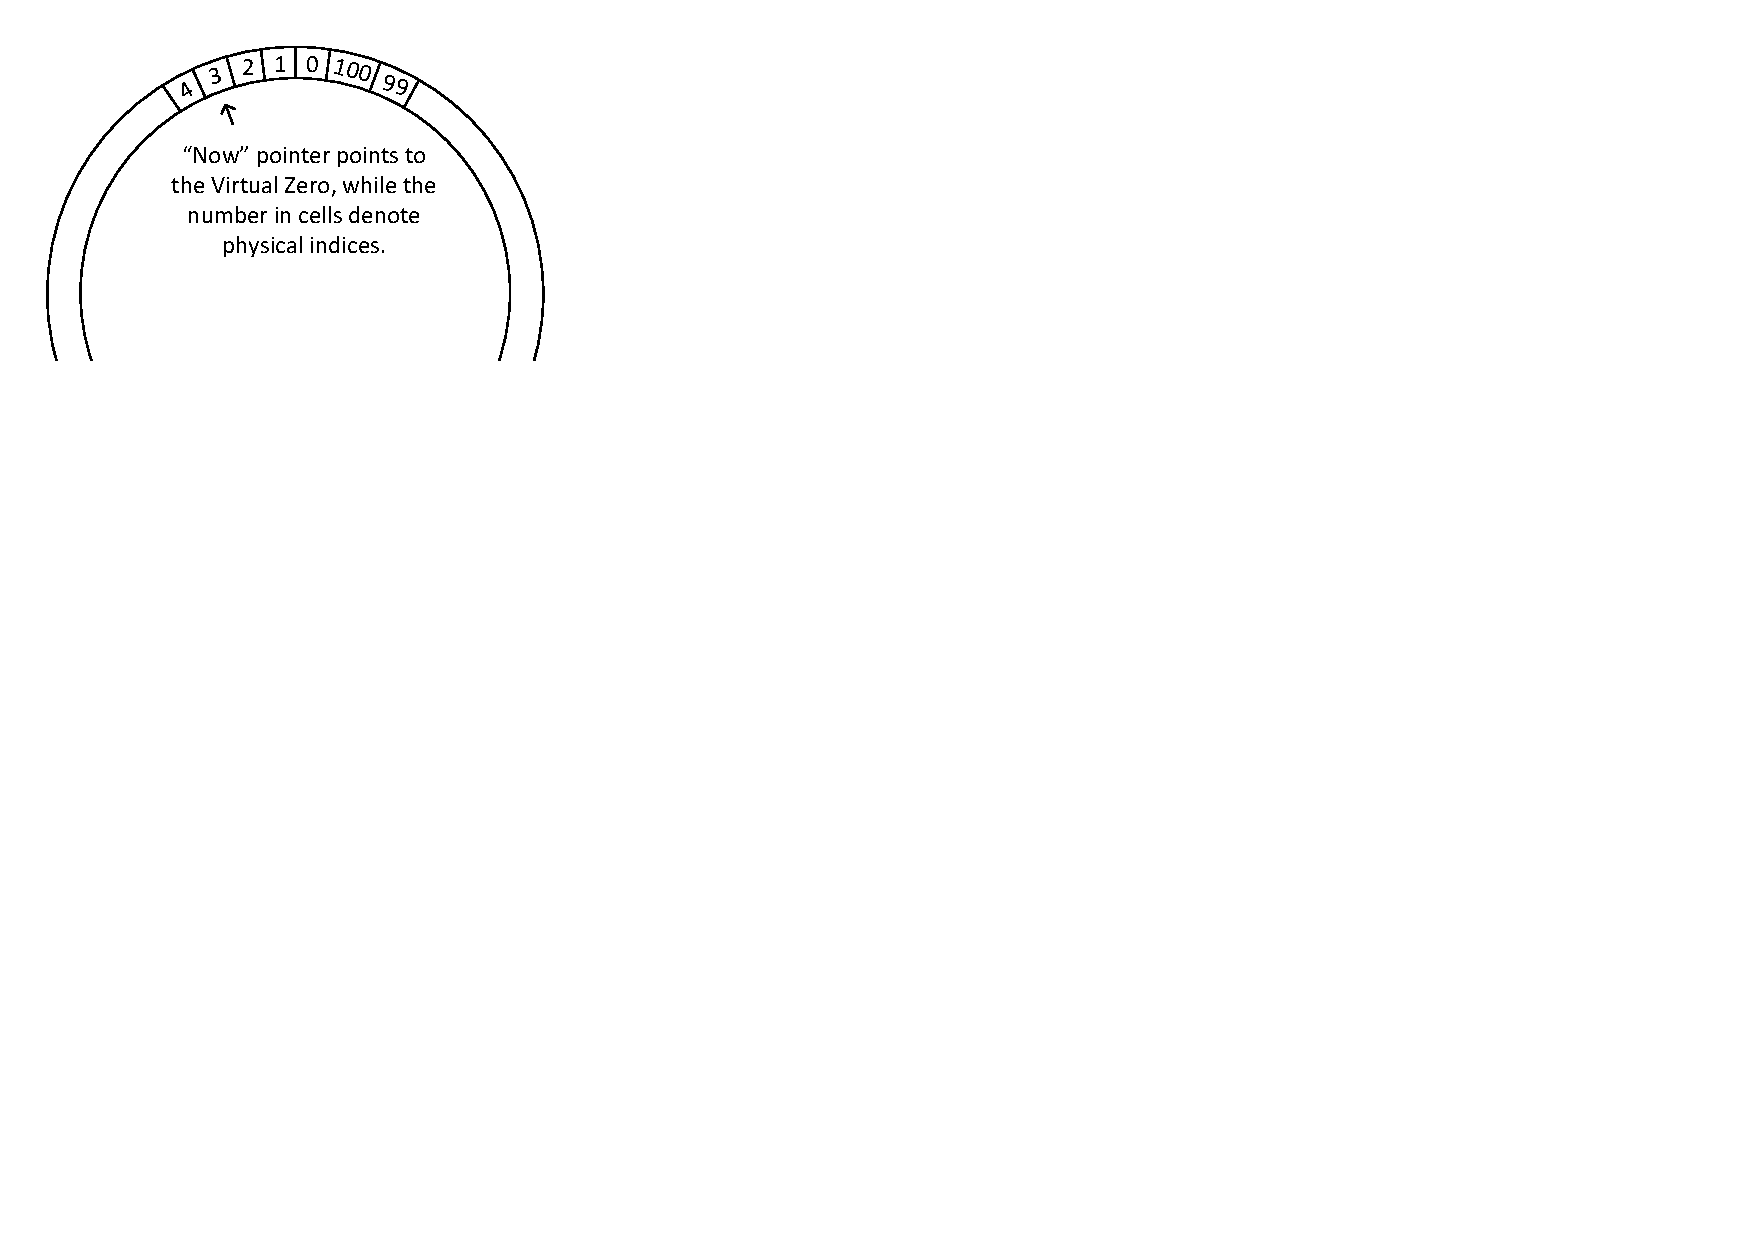
\includegraphics[scale=0.85]{circle.pdf}
	\caption{An illustration of a circular array. The \texttt{CircularArr} instance in \emph{NNBot} contains 101 snapshots, although the code itself is general-purpose.}
	\label{fig:circle}
\end{figure}

\subsection{Class EnemyModel}
\label{sec:model}

Class \texttt{EnemyModel} is the core of the neural-targeting system. An \texttt{EnemyModel} instance maintains the name of the enemy, an \texttt{ANN} instance with 60 input neurons, 60 hidden neurons, and 20 output neurons, and a circular array of snapshots. The class itself implements the \texttt{Externalizable} interface. When a battle ends, the name of the enemy and the neural network are written to a file that is specific to this enemy, while the knowledge base is abandoned.

This class provides an important function \texttt{predict({\small{AdvancedRobot, ScannedRobotEvent}})}. This function is called from the main controller once a \texttt{ScannedRobotEvent} is received. And since the main controller uses one-on-one radar locking \cite{radar_lock}, this function is called on every time tick. Since one tick is too short for the enemy to do anything meaningful, the neural-targeting system works on the time unit \emph{instant}, which equals five Robocode time ticks. Upon this function being called, the system does the following things:

\begin{enumerate}[itemsep=0mm]
\item A \texttt{Snapshot} instance is created and added to the knowledge base.
\item The system queries the knowledge base for snapshots of 20 to 11 instants ago. These snapshots are merged to an input vector. The knowledge base is also queried for snapshots of 9 to 0 instants ago. From these snapshots, the heading and velocity of the enemy are extracted, and are merged to an output vector. The input and output vectors are equivalent to the previous 10 and future 10 snapshots at the time of 10 instants ago, as illustrated by \hyperref[fig:time]{figure~\ref{fig:time}}. With these two vectors, the neural network gets trained.
\item The system queries the knowledge base for the 10 most recent snapshots. These snapshots are merged to an input vector, and are fed into the neural network. The output of the neural network, then, are the expected velocity and heading of the enemy in the next 10 instants.
\item The system then transforms these expected velocity and heading to expected enemy locations in Cartesian coordinates, and returns them to the main controller.
\end{enumerate}

\begin{figure}[h]
	\centering
	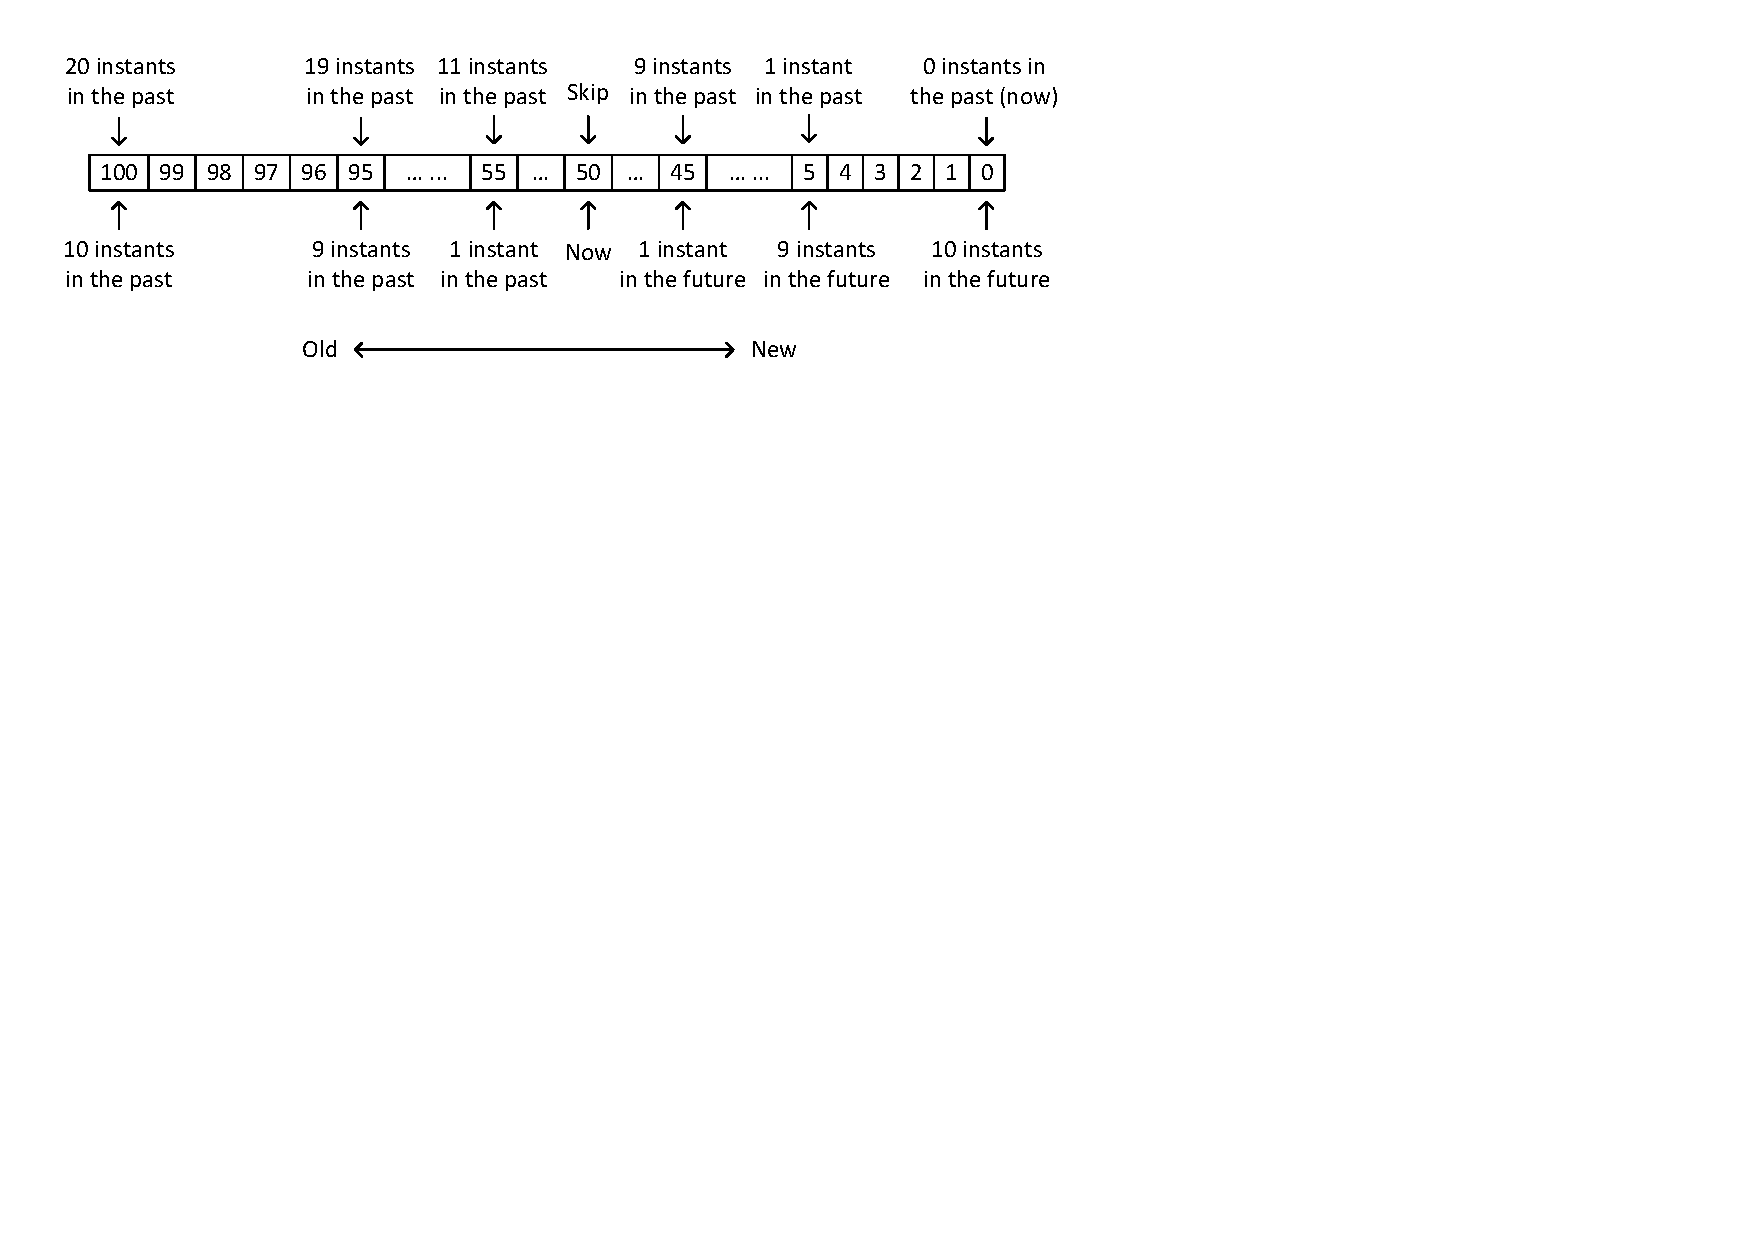
\includegraphics[scale=0.85]{time.pdf}
	\caption{An illustration of time travel. Numbers in the cells denote the time a snapshot is taken. The rightmost cell contains the snapshot taken on the current time tick, while the leftmost cell contains the snapshot taken 100 ticks ago. Notations above the cells are from the point of view of now, while notations below the cells are from the point of view of 10 instants ago.}
	\label{fig:time}
\end{figure}

\subsection{Class NNBot}

Class \texttt{NNBot} is the main controller of the bot. Besides using an \texttt{EnemyModel} instance as the neural-targeting system, it uses one-on-one radar locking as the radar control, and a movement controller adapted from \emph{RandomMovementBot} \cite{random_movement_bot}.

Once a \texttt{ScannedRobotEvent} is received, the agent forwards it to the neural-targeting system. Meanwhile, it calculates the time it takes the bullet to arrive at the current location of the enemy. With the returned sequence of predicted locations, the system finds the nearest two instants where the expected location of the enemy is defined. The target, then, is a linear combination of these two points. Finally, the system fires a bullet with minimum power to the target. The minimum power allows the bullet to travel faster, and therefore have a higher chance of hitting the enemy. Winning the battle, on the other hand, is not a priority of \texttt{NNBot}.

One extra feature of this class is to paint the predicted location of the enemy. The expected locations of the enemy in the next 10 instants are painted as red crosses, while the chosen target is painted as a white cross.

\section{Experiments}

\subsection{Against \emph{SpinBot}}
\label{sec:spin}

\emph{SpinBot} is a library bot that performs circular movement and head-on targeting. It is the first bot that I tested \emph{NNBot} against, since I' like to know if artificial neural network can handle discontinuities, as shown in \hyperref[fig:discontinuity]{figure~\ref{fig:discontinuity}}:

\begin{figure}[h]
	\centering
	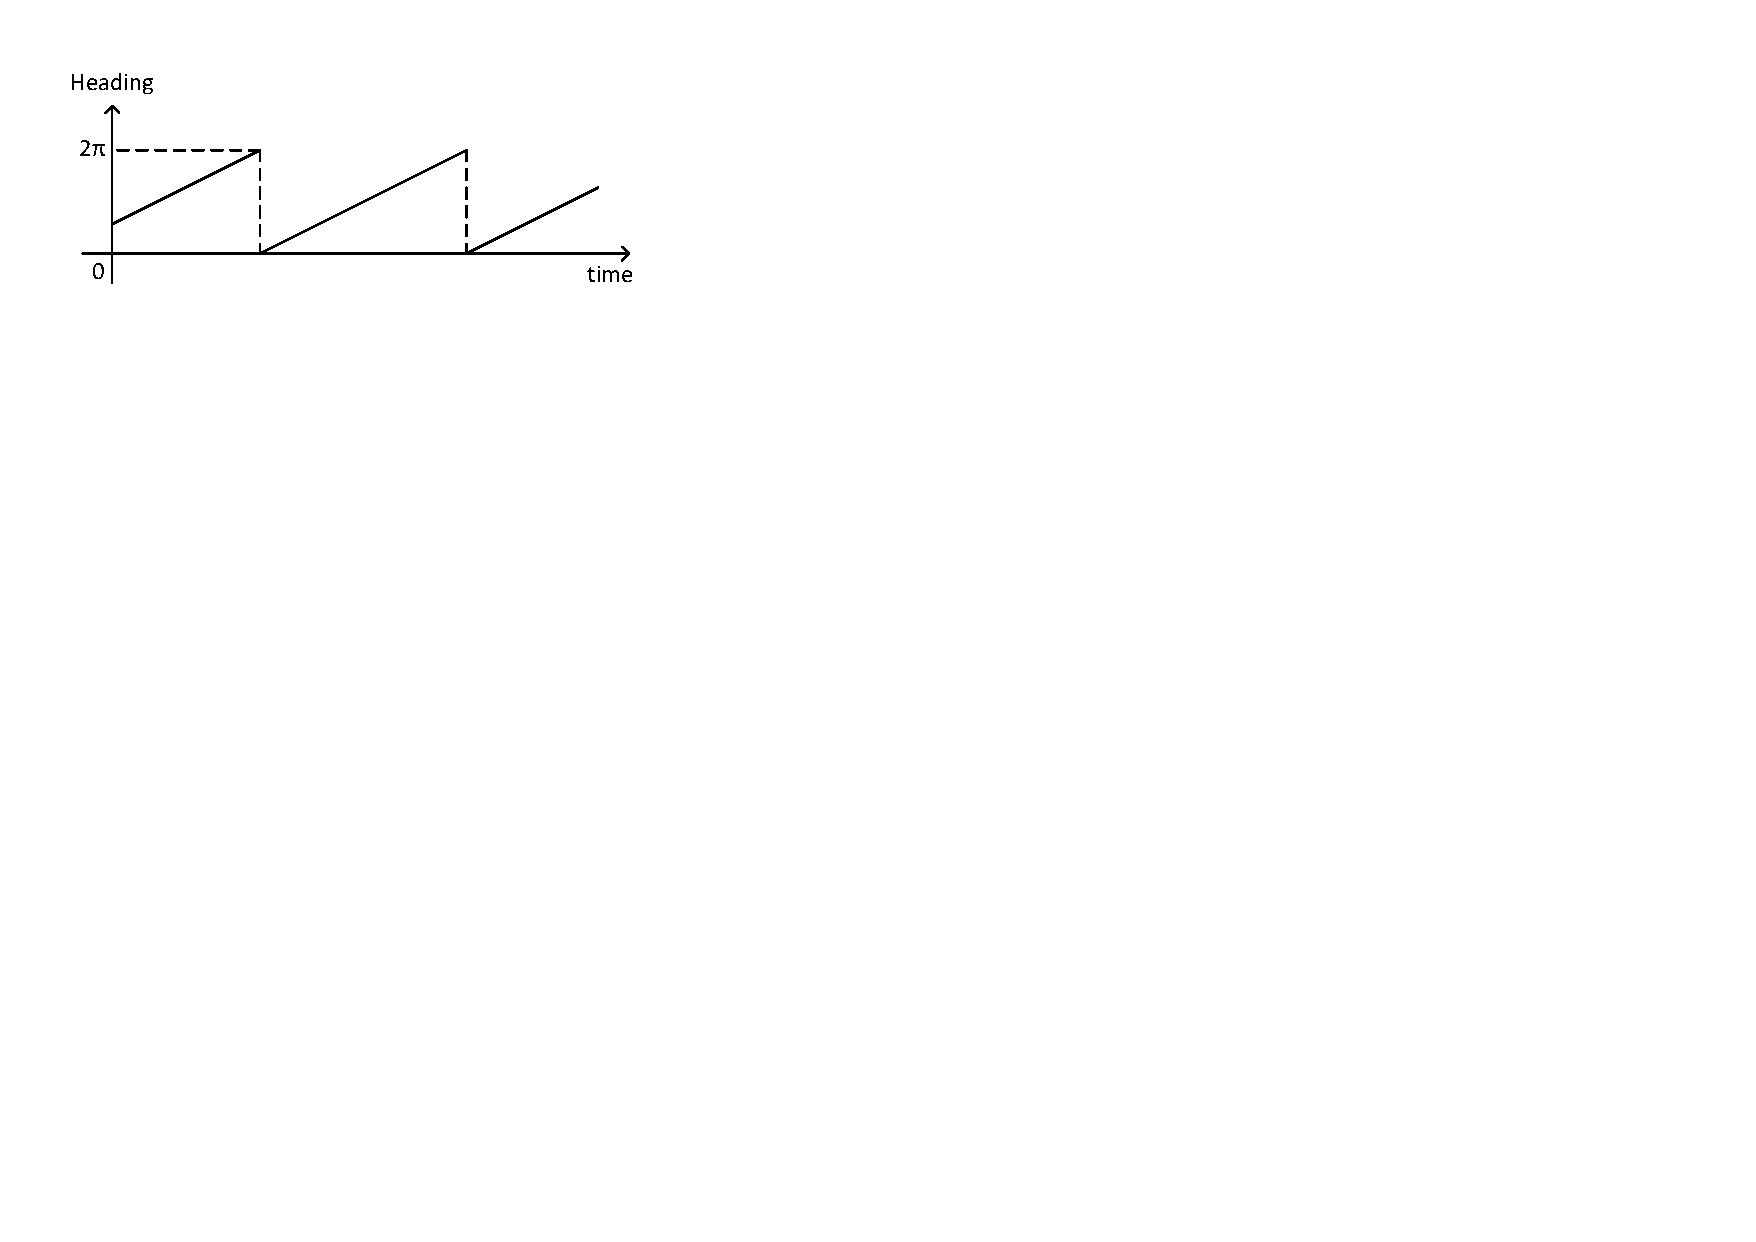
\includegraphics[scale=0.85]{discontinuity.pdf}
	\caption{The heading of \emph{SpinBot}, from the point of view of \emph{NNBot}, is not continuous: It increases linearly to $2\pi,$ drops to 0, and starts climbing again. The velocity of \emph{SpinBot}, on the other hand, is simply a constant.}
	\label{fig:discontinuity}
\end{figure}

It turned out that the answer is more than just yes or no. \emph{BigBrain}, with 300 input neurons and 100 output neurons, is unable to learn this function at all. During the 1000 rounds of training, its predicted enemy heading keeps alternating between 0 and $2\pi$, which are in fact the same. As a result, its predicted positions of the enemy is constantly pointing straight north. \emph{NNBot}, on the other hand, is able to learn this function within one round by replacing the discontinuity with a sharp decrease. However, the neural-targeting system of \emph{NNBot} learns so fast that it soon starts to suffer from overfitting. The overfitted prediction of heading, similar to \emph{BigBrain}, tends to alternate between 0 and $2\pi$.

While investigating when the neural-targeting system of \emph{NNBot} starts to overfit, the eva-luation of performance became an unexpected problem. Originally, \emph{NNBot} maintains a fired bullet counter and a bullet hit counter. These two counters allow the performance of \emph{NNBot} to be evaluated by bullet hit rate once every 100 time ticks. However, during the experiment, I noticed that when the predicted positions of the enemy is already clearly overfitting, the bullet hit rate remains unaffected. The major impact on bullet hit rate, though, comes from the relative bearing between the two bots: If \emph{NNBot} is on the north or south of \emph{SpinBot}, the bullet hit rate is around $40\%.$ But if \emph{NNBot} is on the east or west of \emph{SpinBot}, the bullet hit rate rarely exceeds $25\%.$ Therefore, it is concluded that noise overwhelms signal in bullet hit rate statistics. In the following discussions, the performance of the neural-targeting system is primarily judged by inspecting the predicted locations of the enemy. Screenshots of a nice prediction and an overfitted prdiction are shown in \hyperref[fig:spin]{figure~\ref{fig:spin}}.

\begin{figure}[h]
	\centering
	\begin{subfigure}
		\centering
		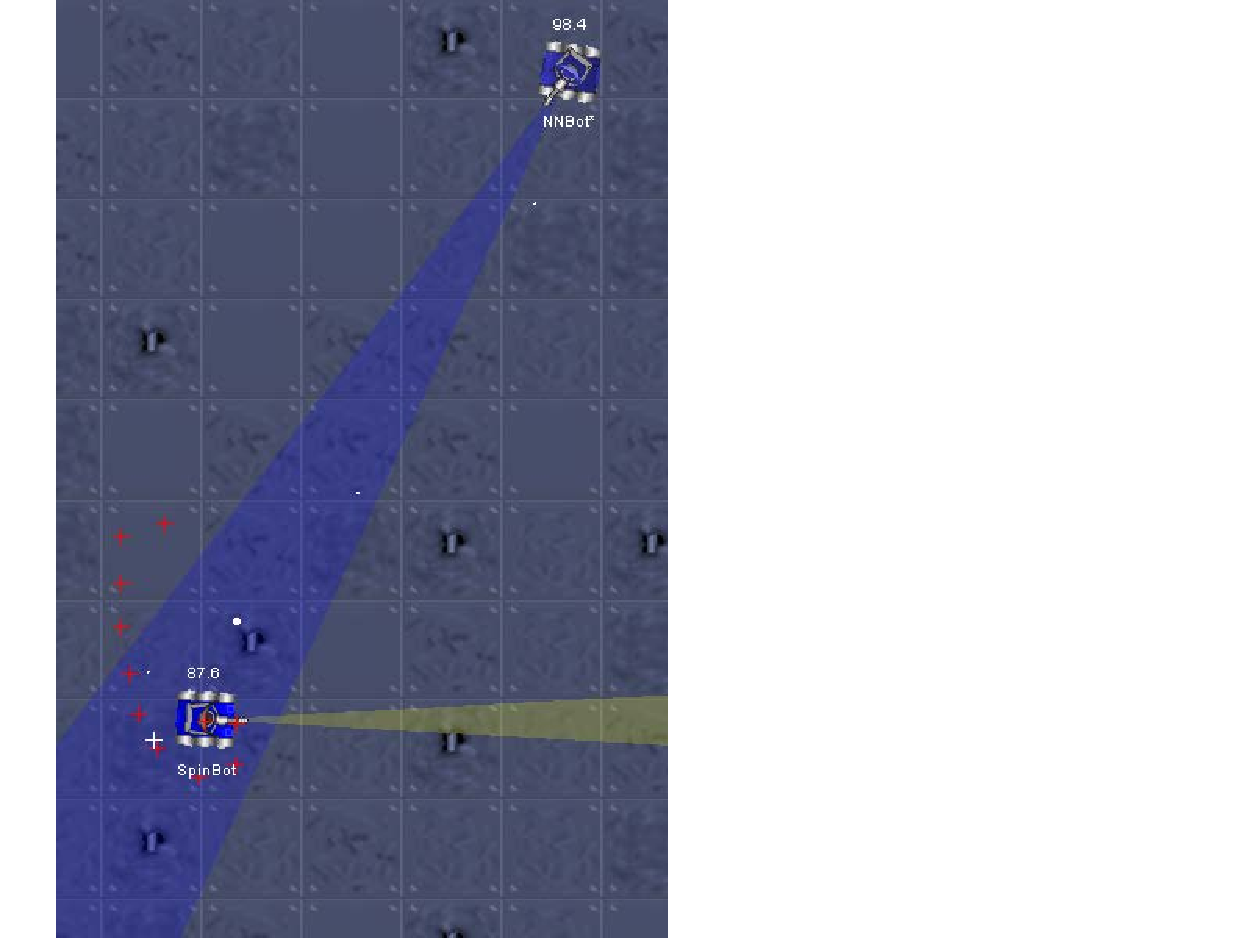
\includegraphics[scale=0.65]{spinbot_good.pdf}
	\end{subfigure}
	\begin{subfigure}
		\centering
		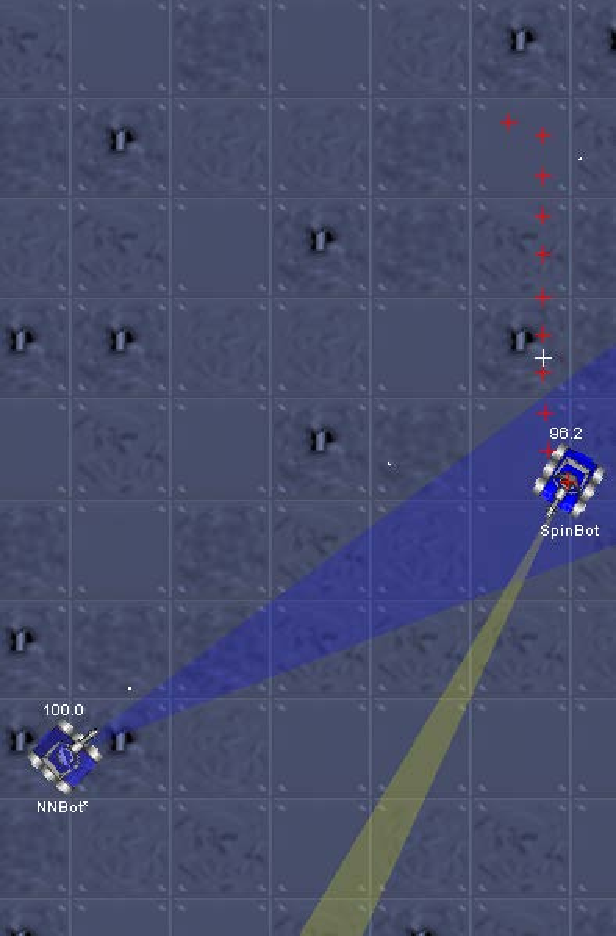
\includegraphics[scale=0.65]{spinbot_bad.pdf}
	\end{subfigure}
	\caption{Two screenshots of \emph{NNBot} against \emph{SpinBot}. The prediction on the left looks relatively good, while the prediction on the right is clearly overfitted.}
	\label{fig:spin}
\end{figure}

\subsection{Against \emph{Crazy}}

\emph{Crazy} is my favourite library bot. It performes circulat movement, but changes direction when it finishes turnning 90 degrees, or when it hits the wall or another robot. Such design allows it to have very random behaviours (without using a random number generator), and therefore, making the prediction of its future movement a challenging task. The neural-targeting system of \emph{NNBot} does not perform too well against \emph{Crazy}, with the prediction of enemy positions often failing to point to a clear direction. \hyperref[fig:crazy]{Figure~\ref{fig:crazy}} illustrates the statistics of bullet hit rate in a consecutive 400 rounds, which is even lower than the bullet hit rate of a head-on targeting bot with the same movement control. The reason for such a low bullet hit rate is twofold: First, the neural-targeting system of \emph{NNBot} can take as long as 50 rounds to adapt to a change of direction, and by that time, \emph{Crazy} might have already changed its direction again. Second, artificial neural network may be naturally inefficient to learn a chaotic function, as \cite{ann_robocode} shows very similar results of a neural-targeting bot against \emph{Crazy}.

\begin{figure}[h]
	\centering
	\begin{subfigure}
		\centering
		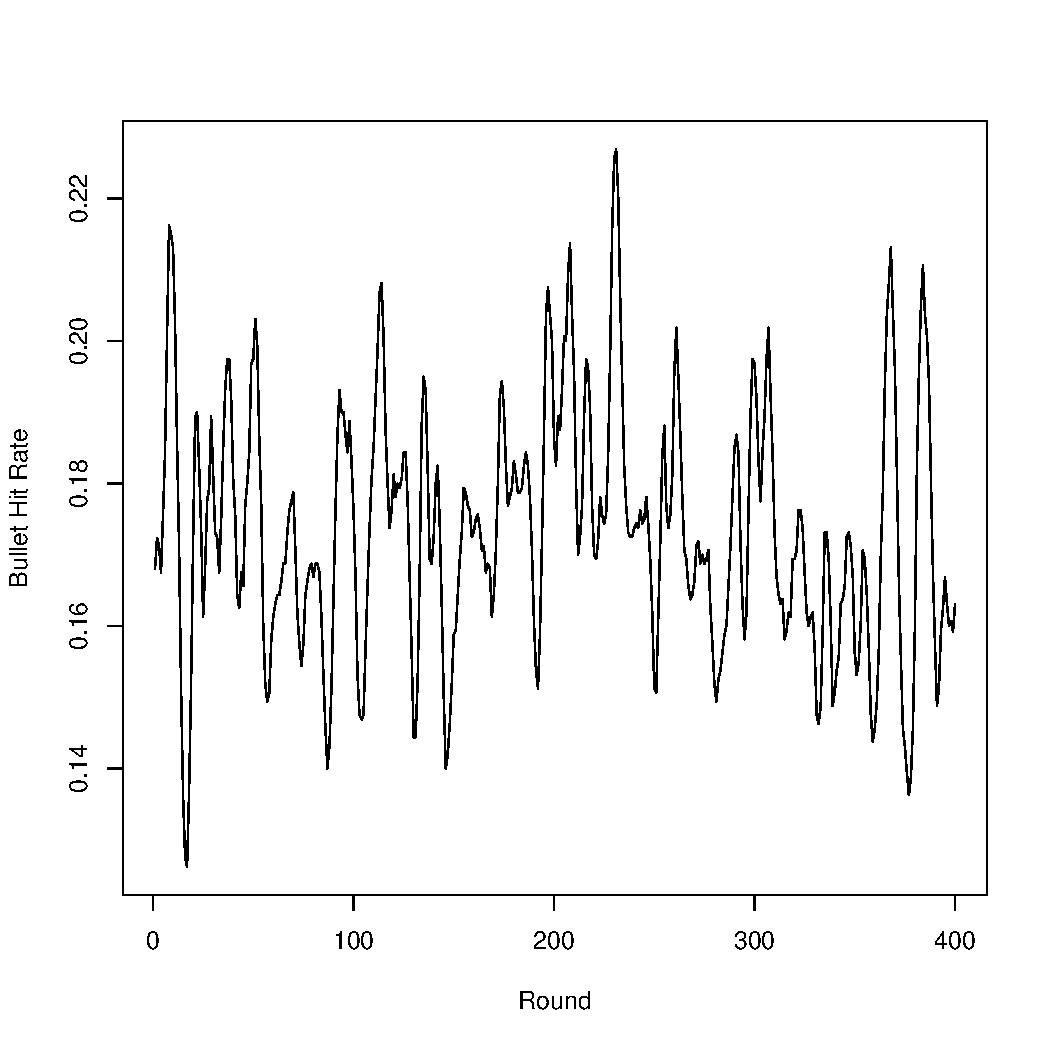
\includegraphics[scale=0.45]{crazy_line.pdf}
	\end{subfigure}
	\begin{subfigure}
		\centering
		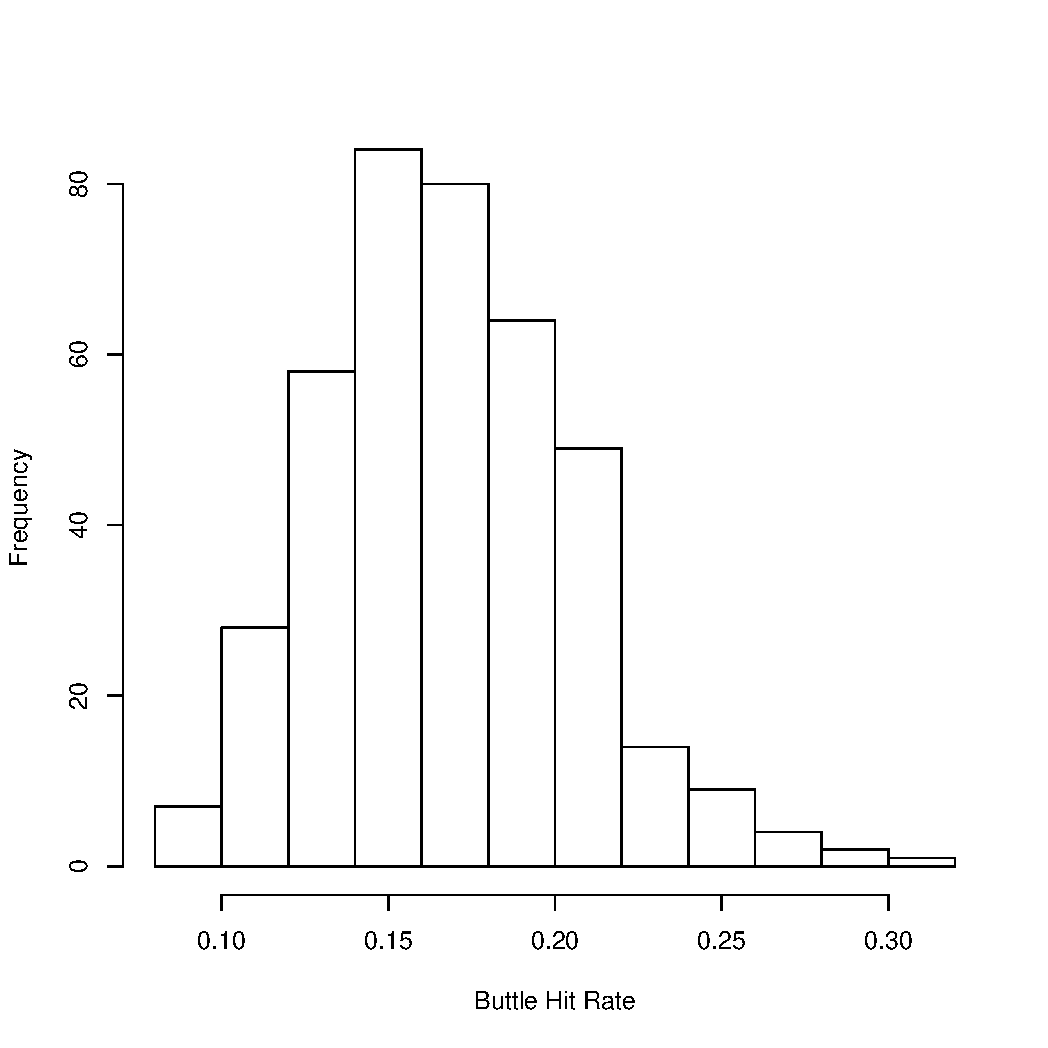
\includegraphics[scale=0.45]{crazy_hist.pdf}
	\end{subfigure}
	\caption{Long-term hit rate statistics of \emph{NNBot} against \emph{Crazy}. The line chart on the left plots bullet hit rate against the number of rounds, and the histogram on the right shows that the bullet hit rate follows a normal distribution.}
	\label{fig:crazy}
\end{figure}

\subsection{Against \emph{Corners}}

\emph{Corners} created the only problem that I havn't been able to explain. Its strategy is to go to a corner, stay there, and shoot its enemy. Since it stays still during the most of the times, the neural-targeting system of \emph{NNBot} can achieve a buttlet hit rate higher than $85\%.$ However, when \emph{Corners} is in the bottom-left corner, i.e.\ when its X and Y coordinates are both close to 0, the neural-targeting system of \emph{NNBot} has a certain chance of completely failing to aim: The predicted heading and velocity both stablizes at some constant, as shown in \hyperref[fig:corners]{figure~\ref{fig:corners}}.

\begin{figure}[h]
	\centering
	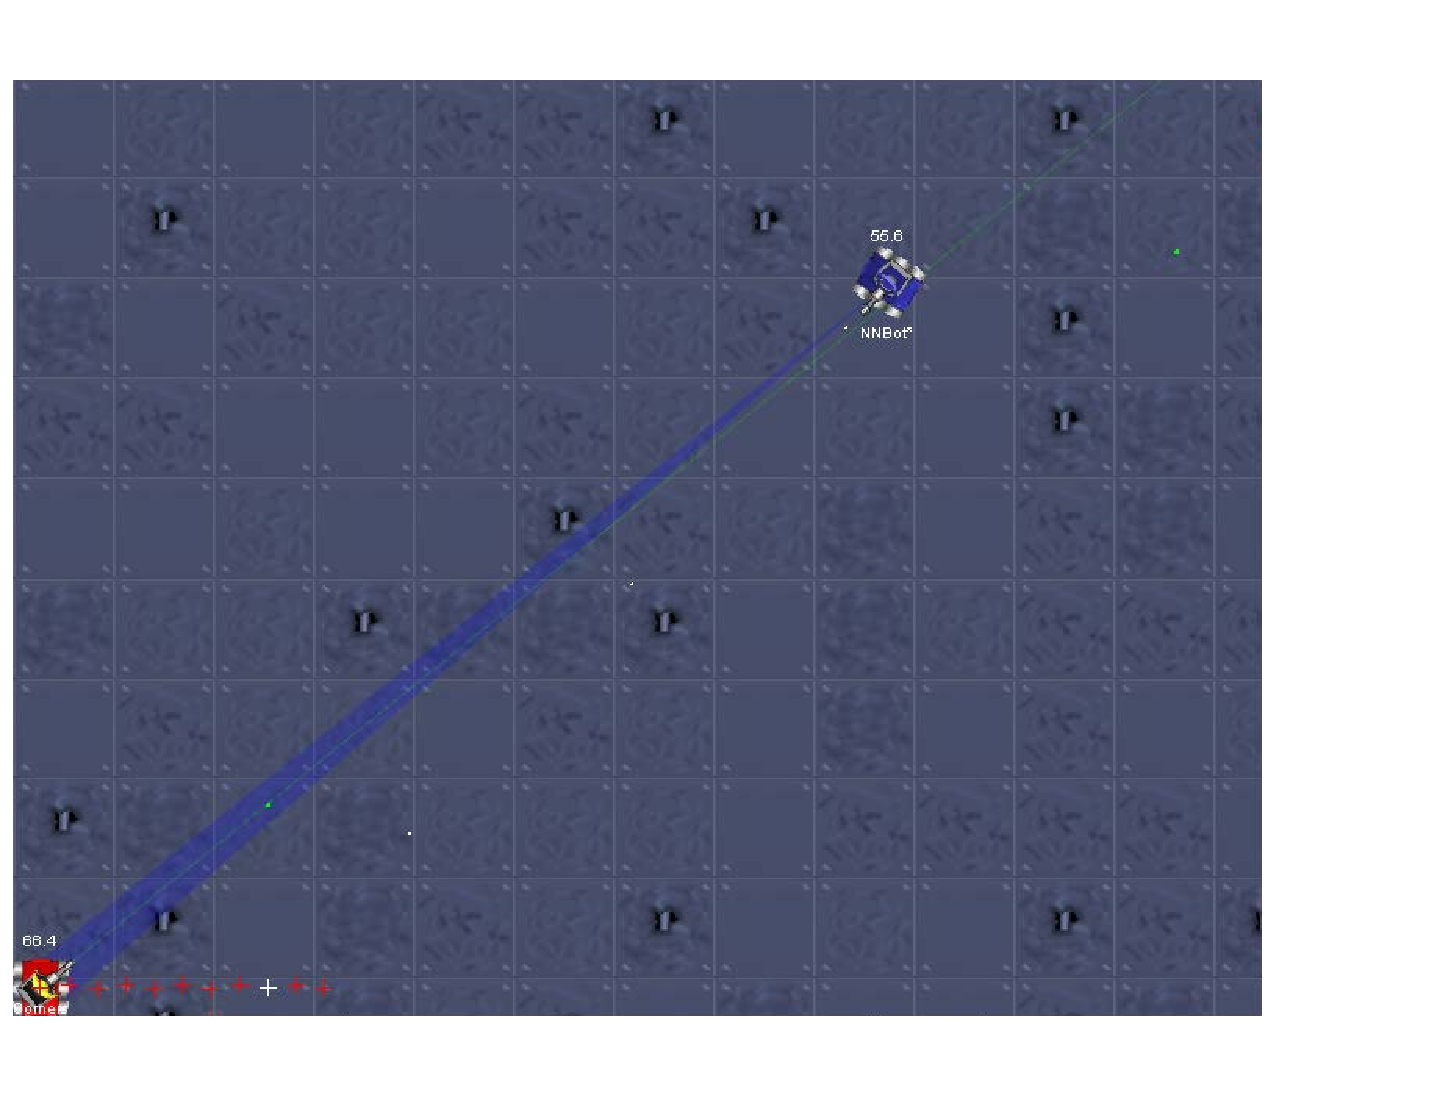
\includegraphics[scale=0.65]{corners.pdf}
	\caption{The problem with \emph{Corners}. The predicted heading stablizes at about $\pi/2,$ and the predicted velocity stablizes at about 3.4 pixels/tick.}
	\label{fig:corners}
\end{figure}

\clearpage

\subsection{Against \emph{RandomMovementBot}}

\emph{RandomMovementBot}, as its name tells, performs random movement while heading almost perpendicular to the enemy. In other words, from its enemy's point of view, it's constantly performing linear lateral movement. This should give the neural-targeting system of \emph{NNBot} an advantage. However, like the case of \emph{Crazy}, \emph{NNBot} does not perform well against random behaviours. A statistics of bullet hit rate in a consecutive 400 rounds is shown in \hyperref[fig:random]{figure~\ref{fig:random}}. Unlike the case of \emph{Crazy}, though, the bullet hit rate of \emph{NNBot} leads that of head-on targeting by more than a standard deviation.

\begin{figure}[htb]
	\centering
	\begin{subfigure}
		\centering
		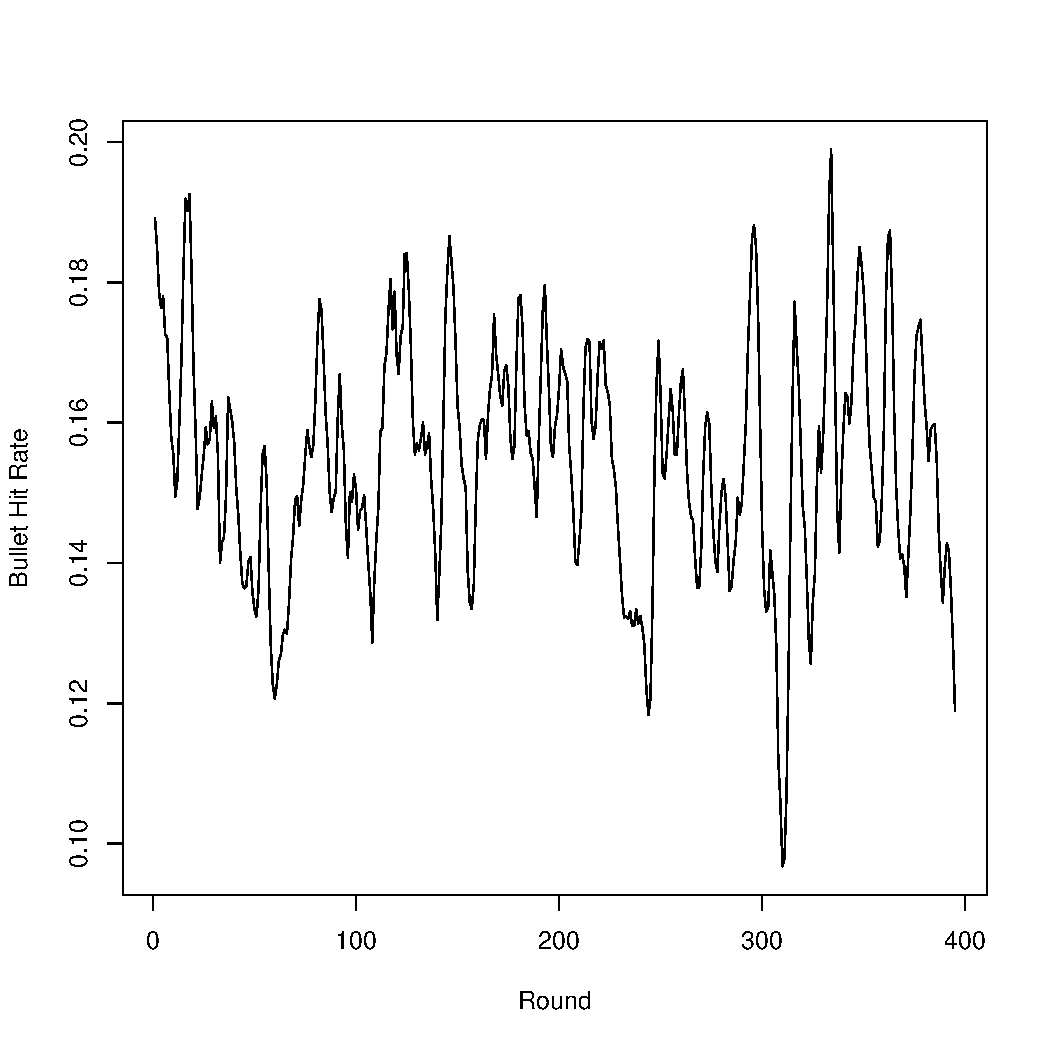
\includegraphics[scale=0.4]{random_line.pdf}
	\end{subfigure}
	\begin{subfigure}
		\centering
		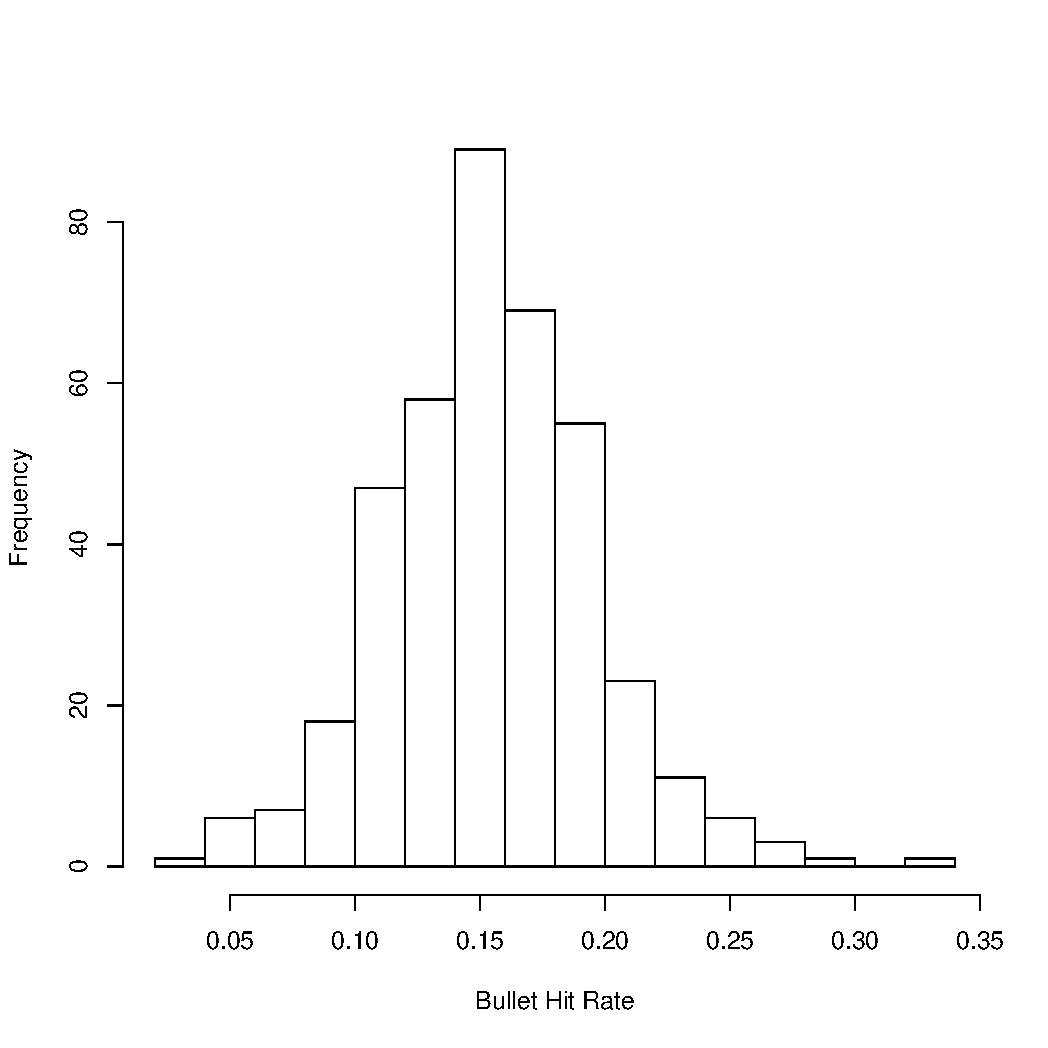
\includegraphics[scale=0.4]{random_hist.pdf}
	\end{subfigure}
	\caption{Long-term hit rate statistics of \emph{NNBot} against \emph{RandomMovementBot}. I haven't been able to find, as a benchmark, any test results of a neural-targeting bot against \emph{RandomMovementBot}.}
	\label{fig:random}
\end{figure}

It is also noteworthy that the behaviour of the neural targeting system of \emph{NNBot} is changing during its learning process. For most of the times, all predicted locations lie on the same line, i.e.\ the neural-targeting system tends to believe that the heading of \emph{RandomMovementBot} stays constant. During the initial period of training, predicted locations of the enemy tend to follow the current direction of the enemy. However, after sufficient amount of training, predicted locations of the enemy start to alternate between the two opposite directions. In other words, it starts to believe that \emph{RandomMovementBot} is going to change its direction somewhere in the future. Given that \emph{RandomMovementBot} has a 0.05 chance to change its direction of acceleration in any time tick, I should conclude that this is a clear sign of a learning system.

\section{Conclusion}

The result of \emph{NNBot} is, again, a mixture of good and bad. On the good side, \emph{NNBot} proved that with a properly designed training algorithm, a back-propagation neural network is not only able to learn the movement of various Robocode agents, but also able to learn very fast. On the bad side, though, the overfit problem can seriously affect the performance of the neural-targeting system, yet they seem to be inevitable against some certain opponents.

Although the code of \emph{NNBot} is designed such that the neural-targeting system can be replaced, there are still two topics that worth exploration under the current framework. First, it shall be greatly beneficial to the firing coltroller if the confidence of the neural network output can be taken into account \cite{ann_confidence}. Second, although it has been shown that cooperation can be evolved from even simple rules \cite{cooperation}, no one has tried to evolve teamwork behaviours in Robocode. The biggest obstacle of this idea shall be the size of the search space, and whether or not the neural network will be too complex to learn effectively.

\bibliographystyle{plain}
\bibliography{Report}

\end{document}
